%LTeX: language=it

\subsection{UC 28 - Sincronizzazione contatti} \label{sec:UC28}
    
    \begin{itemize}
        \item \textbf{Attore principale}: MUA;
        \item \textbf{Descrizione}: il MUA richiede la sincronizzazione con i contatti del sistema;
        \item \textbf{Precondizioni}: l’account che il MUA gestisce è registrato nel sistema, ha una connessione aperta con il sistema ed è autenticato;
        \item \textbf{Postcondizioni}: i contatti sono stati sincronizzati;
        \item \textbf{Scenario principale}:
            \begin{enumerate}
                \item il MUA trasmette l'id dell'account (\hyperref[sec:UC28.1]{UC28.1});
                \item il MUA trasmette gli id dei contatti da aggiornare (\hyperref[sec:UC28.2]{UC 28.2});
                \item il MUA trasmette le proprietà dei contatti da aggiornare (\hyperref[sec:UC28.3]{UC 28.3});
                \item il sistema invia al MUA gli aggiornamenti;
            \end{enumerate}
        \item \textbf{Inclusioni}: nessuna;
        \item \textbf{Generalizzazioni}: nessuna;
        \item \textbf{Estensioni}: nessuna;
    \end{itemize}

    \begin{figure}[H]
        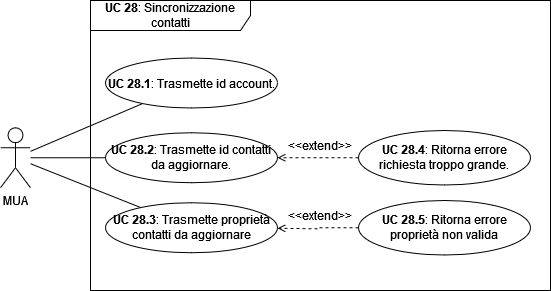
\includegraphics[width=0.85\textwidth]{sections/uc_imgs/UC28.png}
        \centering
        \caption{Sottocasi d'Uso di UC 28}
    \end{figure}

    \subsubsection{UC 28.1 - Trasmette id account} \label{sec:UC28.1}
    \begin{itemize}
        \item \textbf{Attore principale}: MUA;
        \item \textbf{Descrizione}: il MUA invia al sistema l'id dell'account associato all'utente;
        \item \textbf{Precondizioni}: il MUA sta usando la funzionalità di sincronizzazione contatti;
        \item \textbf{Postcondizioni}: il sistema conosce l'id dell'account;
        \item \textbf{Scenario principale}:
            \begin{enumerate}
                \item il MUA trasmette l'id dell'account associato all'utente al sistema;
            \end{enumerate}
        \item \textbf{Inclusioni}: nessuna;
        \item \textbf{Generalizzazioni}: nessuna;
        \item \textbf{Estensioni}: nessuna;
    \end{itemize}

    \subsubsection{UC 28.2 - Trasmette id contatti da aggiornare} \label{sec:UC28.2}
    \begin{itemize}
        \item \textbf{Attore principale}: MUA;
        \item \textbf{Descrizione}: il MUA invia al sistema gli id dei contatti da aggiornare;
        \item \textbf{Precondizioni}: il MUA sta usando la funzionalità di sincronizzazione dei contatti;
        \item \textbf{Postcondizioni}: il sistema conosce gli id dei contatti da aggiornare;
        \item \textbf{Scenario principale}:
            \begin{enumerate}
                \item il MUA trasmette gli id dei contatti da aggiornare;
            \end{enumerate}
        \item \textbf{Inclusioni}: nessuna;
        \item \textbf{Generalizzazioni}: nessuna;
        \item \textbf{Estensioni}:
            \begin{enumerate}[label=\alph*.]
                \item la quantità di contatti da aggiornare supera la quantità massima di richieste al server:
                \begin{enumerate}[label=\arabic*.]
                    \item il sistema ritorna un errore al MUA di richiesta troppo grande (\hyperref[sec:UC28.4]{UC 28.4}).
                \end{enumerate}
            \end{enumerate}
    \end{itemize}


    \subsubsection{UC 28.3 - Trasmette proprietà contatti da aggiornare} \label{sec:UC28.3}
    \begin{itemize}
        \item \textbf{Attore principale}: MUA;
        \item \textbf{Descrizione}: il MUA invia al sistema le proprietà dei contatti da aggiornare;
        \item \textbf{Precondizioni}: il MUA sta usando la funzionalità di sincronizzazione dei contatti;
        \item \textbf{Postcondizioni}: il sistema conosce quali sono le proprietà dei contatti da aggiornare;
        \item \textbf{Scenario principale}:
            \begin{enumerate}
                \item il MUA trasmette le proprietà dei contatti da aggiornare;
            \end{enumerate}
        \item \textbf{Inclusioni}: nessuna;
        \item \textbf{Generalizzazioni}: nessuna;
        \item \textbf{Estensioni}:
            \begin{enumerate}[label=\alph*.]
                \item le proprietà dei contatti da aggiornare non sono valide:
                \begin{enumerate}[label=\arabic*.]
                    \item il sistema ritorna un errore al MUA di proprietà non valida (\hyperref[sec:UC28.5]{UC 28.5}).
                \end{enumerate}
            \end{enumerate}
    \end{itemize}


    \subsubsection{UC 28.4 - Ritorna errore richiesta troppo grande} \label{sec:UC28.4}
    \begin{itemize}
        \item \textbf{Attore principale}: MUA;
        \item \textbf{Descrizione}: il MUA riceve l'errore che la quantità dei contatti da aggiornare supera la quantità massima di richieste al server;
        \item \textbf{Precondizioni}: il MUA ha inviato gli id dei contatti da aggiornare;
        \item \textbf{Postcondizioni}: il sistema non invia gli aggiornamenti e il MUA viene notificato che il numero dei contatti da aggiornare è eccessivo;
        \item \textbf{Scenario principale}:
            \begin{enumerate}
                \item il sistema verifica la quantità di richieste;
                \item il sistema rileva che il numero di richieste supera la soglia massima consentita;
                \item il sistema non invia gli aggiornamenti e notifica il MUA dell'eccesso di richieste;
            \end{enumerate}
        \item \textbf{Inclusioni}: nessuna;
        \item \textbf{Generalizzazioni}: nessuna;
        \item \textbf{Estensioni}: nessuna.
    \end{itemize}

    \subsubsection{UC 28.5 - Ritorna errore proprietà non valida} \label{sec:UC28.5}
    \begin{itemize}
        \item \textbf{Attore principale}: MUA;
        \item \textbf{Descrizione}: il MUA riceve l'errore che la proprietà dei contatti da aggiornare non è valida;
        \item \textbf{Precondizioni}: il MUA ha inviato la proprietà dei contatti da aggiornare;
        \item \textbf{Postcondizioni}: il sistema non invia gli aggiornamenti e il MUA viene notificato che la proprietà dei contatti da aggiornare non è valida;
        \item \textbf{Scenario principale}:
            \begin{enumerate}
                \item il sistema verifica la validità della proprietà trasmessa e trova un errore;
                \item il sistema non invia gli aggiornamenti e notifica il MUA dell'errore;
            \end{enumerate}
        \item \textbf{Inclusioni}: nessuna;
        \item \textbf{Generalizzazioni}: nessuna;
        \item \textbf{Estensioni}: nessuna.
    \end{itemize}